\section{Analysing the pipe and filter software architecture and the monitoring system built using it}
\label{sec:architecture}
The pipe and filter architecture is composed implies that each component of the system is able to read data from a stream and output data to another stream. Components are the filters and the streams are the pipes. Filters should not share state with other filters and should not make assumptions about other filters in the system. Among the properties provided by such an architecture are: simpler understanding of the processing done by a system, by analysing the order of the filters and their responsibilities, filters are easy to reuse, maintain and replace, they support concurrent execution.

For every system the architecture is important because it dictates the means by which scalability can be obtained. Fig. \ref{fig:systemArchitecture} presents the architecture of the system we want to extend. The architecture is an extension of the one presented in \cite{IrimieAndPetcu}. The system is composed of 7 components: "FrontEnd", "Scanner", "Converter", "Presenter", "Remediator", a document database and a message queue. The first five components send messages using the queues and are completely decoupled from one another, from each component perspective the system is only compose of itself and one or more message queues. This decoupling provides grate opportunity for replication and scalability, but it imposes some constraints on the allocation of jobs to replicas of the same component.


\begin{figure*}[ht]
\centering
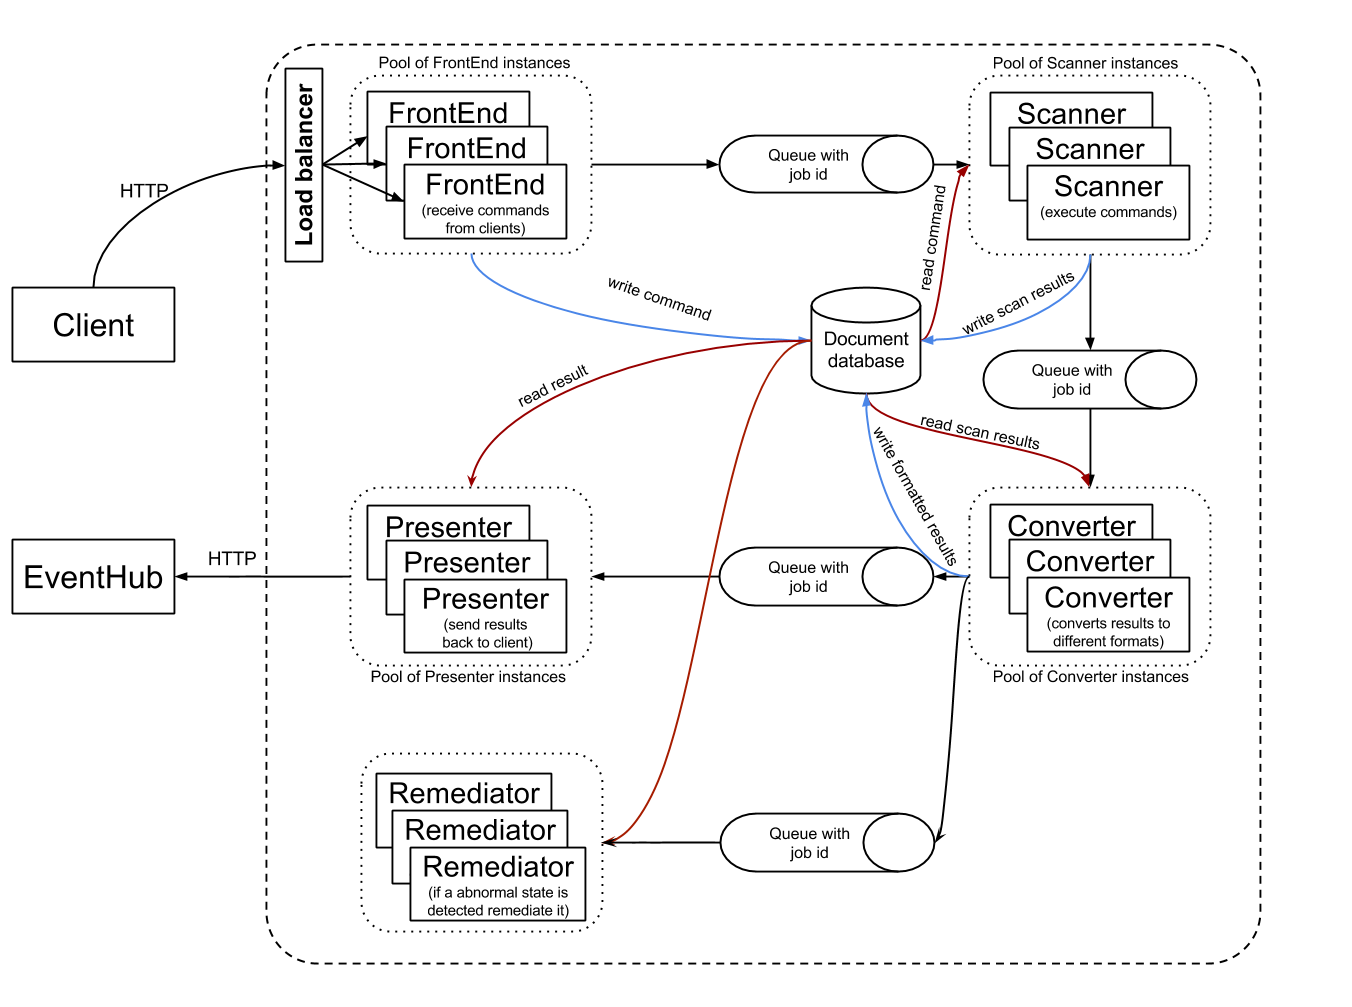
\includegraphics[width=\linewidth]{./img/MonitoringSystemArchitectureRemediation.png}
\caption{Distributed monitoring system architecture}
\label{fig:systemArchitecture}
\end{figure*}

